\documentclass[article,12pt,a4paper]{article}
\usepackage[latin1]{inputenc}
\usepackage[T1]{fontenc} 
\usepackage[english]{babel} 

%\pagestyle{empty
	%\usepackage{emoji}} 
\usepackage{longtable}
\usepackage{enumitem}
\usepackage{alphalph}

\usepackage{amsmath, amsthm}
\newtheorem{theorem}{Theorem}
\newtheorem{proposition}{Proposition}
\newtheorem{lemma}{Lemma}
\newtheorem*{proof*}{Proof}
\newtheorem{definition}{Definition}

\newtheorem{exercise}{Exercise}
\newtheorem{question}{Question}

\newtheorem{example}{Example}

\newtheorem{remark}{Remark}

\usepackage[a4paper,left=1.5cm, right=1.5cm,top=1.5cm,bottom=1.5cm]{geometry}
\setlength{\columnsep}{1.2cm}

%\usepackage{cancel}
\usepackage{bm}
\usepackage{amssymb,amsfonts}
\usepackage{mathrsfs}
\usepackage{color}
%\usepackage{hyperref}
\usepackage{dsfont}
\usepackage{graphicx}
\usepackage{algorithmicx}
\usepackage[ruled]{algorithm}
\usepackage{algpseudocode}
\usepackage{marginnote}

\usepackage{tikz}
\usetikzlibrary{shapes.geometric, arrows, positioning}


\newcommand{\Ptr}{\mathcal P^{\rm tr}}
\newcommand{\tr}{{\rm tr}}
\newcommand{\N}{\mathbb N}
\newcommand{\calN}{\mathcal N}
\newcommand{\bP}{\bold P}
\newcommand{\calK}{\mathcal K}
\newcommand{\calF}{\mathcal F}
\newcommand{\calH}{\mathcal H}
\newcommand{\calP}{\mathcal P}
\newcommand{\calC}{\mathcal C}
\newcommand{\R}{\mathbb R}
\newcommand{\bX}{\bar X}

\newcommand{\calS}{\mathcal S}

\newcommand{\bQ}{\bold Q}
\newcommand{\bs}{\bold s}
\newcommand\red[1]{\textcolor{red} {#1} }

\title{ \bfseries \Huge {Re-sit exam : stochastic processes}}    
%\vspace{-4cm}        

\date{June $5^{th}$, 2025}       
%\vspace{-4cm}        
%\newcounter{num}
%\Alph{num}


\begin{document}
	% Start the paragraph counter at 1
	
	\paragraph{Problem 1.}
	
	Consider a discrete-time Markov chain (DTMC) $\{X_n\}_{n\in\N}$ whose one-step transition probabilities are shown below.
		\begin{figure}[h]
		\centering
		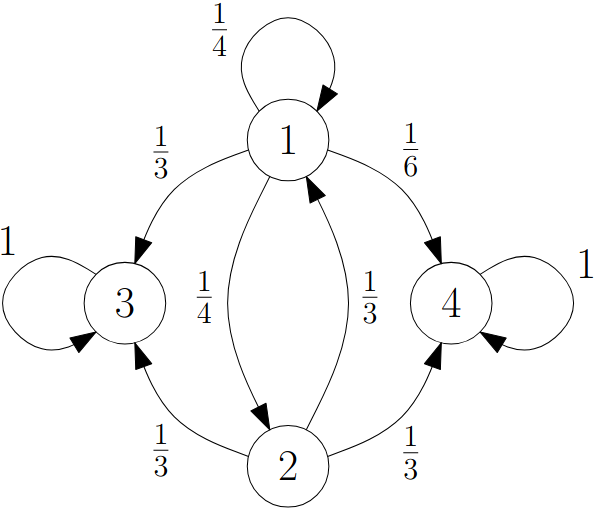
\includegraphics[width=0.3\textwidth]{markov_1.png} 
	\end{figure}
	\begin{enumerate}
		\item\textit{[2 points]}  Classify the states of this DTMC.
		\item\textit{[5 points]}  Suppose that the chain starts at $X_0 = 2$. Find the probability that $X_2 = 4$.
		%\item\textit{[5 points]}  Does the Markov chain converge? Justify your answer.
		\item\textit{[5 points]} What is the probability of eventually visiting state 4, given that the initial state is $X_0 = 1$?
		
	\end{enumerate}
	\medskip
	
		\paragraph{Problem 2.}
	Consider the DTMC over state space $\calS = \{1,2,3\}$ with transition matrix
	\[
	\bQ = \begin{pmatrix}
		\frac{1}{2} & \frac{1}{3} & \frac{1}{6} \\
		\frac{3}{4} & 0 & \frac{1}{4} \\
		0 & 1 & 0
	\end{pmatrix}
	\]
	
	\begin{enumerate}
		\item \textit{[5 points]} Does this Markov chain converge? Justify your answer.
		
		\item \textit{[5 points]} Find the matrix which is the limit of $\bQ^n$ as $n \to \infty$.
		
		\item \textit{[5 points]} Find the mean recurrence time to state 3, i.e., the expected number of transitions it takes to return to state 3, starting from state 3.
	\end{enumerate}
	
	
	\paragraph{Problem 3.}
	The inter-arrival times for cars passing a checkpoint are independent random variables with PDF
	\[
	f_T(t) =
	\begin{cases}
		2e^{-2t}, & t > 0 \\
		0, & \text{otherwise}
	\end{cases}
	\]
	where the inter-arrival times are measured in minutes. The successive experimental values of the durations of these inter-arrival times are recorded on small computer cards. The recording operation occupies a negligible time period following each arrival. Each card has space for three entries. As soon as a card is filled, it is replaced by the next card.
	
	\begin{enumerate}
		\item\textit{[5 points]} Given that no car has arrived in the last four minutes, determine the PMF for random variable $K$, the number of cars to arrive in the next six minutes.
		
		\item\textit{[5 points]} Determine the PDF and the expected value for the total time required to use up the first two computer cards.
	\end{enumerate}
	
	
	\paragraph{Problem 4.}
	\begin{enumerate}
		\item\textit{[5 points]} Is the Metropolis-Hastings algorithm guaranteed to converge to the distribution of interest if we choose a \textbf{reducible} proposal matrix? Justify your answer.
	\end{enumerate}
	
	\paragraph{Problem 5.}
	Consider two copier machines that are maintained by a single repairman. Machine $i\in\{1,2\}$ functions for an exponentially distributed amount of time with mean $1/\gamma_i$, with $\gamma_i>0$, before it breaks down. 
	The repair times for copier $i\in\{1,2\}$ are exponential with mean $1/\beta_i$, with $\beta_i>0$, but the repairman can only work on one machine at a time. 
	Assume that the machines are repaired in the order in which they fail.
	
	We wish to construct a continuous-time Markov chain (CTMC) model of this system, with the goal of finding the long-run proportions of time that each copier is working and the repairman is busy. 
	We use the 5 following states :
	\begin{itemize}
		\item 0 for no copiers failed,
		\item 1 for copier 1 is failed (and copier 2 is working),
		\item 2 for copier 2 is failed (and copier 1 is working),
		\item (1,2) for both copiers down (failed) with copier 1 having failed first and being repaired,
		\item (2,1) for both copiers down with copier 2 having failed first and being repaired.
	\end{itemize}
	The graph of this CTMC is as shown below 
	\begin{figure}[h]
		\centering
		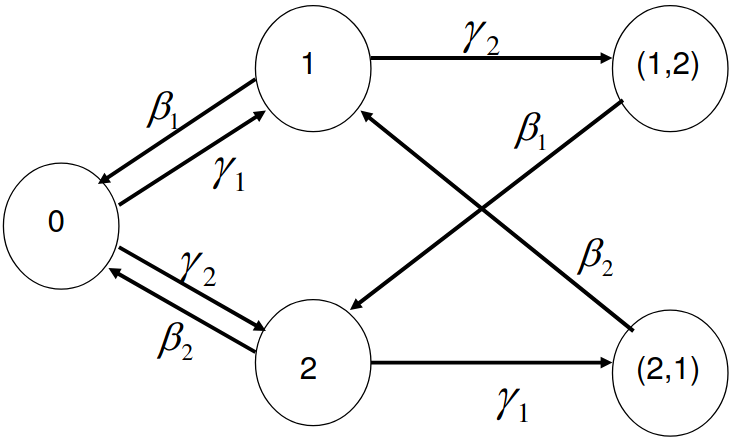
\includegraphics[width=0.35\textwidth]{ctmc_1.png} 
	\end{figure}
	
	\begin{enumerate}
		\vspace{-.1cm}
		\item \textit{[5 points]} Give the infinitesimal generator of this CTMC.
		\item \textit{[5 points]} Does this CTMC have a unique stationary distribution? Justify your answer.
	\end{enumerate}
	Now let us consider an alternative repair strategy: Suppose that copier 1 is more
	important than copier 2, so that it is more important to have it working. Toward that end,
	suppose the repairman always work on copier 1 when both copiers are down. In particular,
	now suppose that the repairman stops working on copier 2 when it is down if copier 1 also
	subsequently fails, and immediately shifts his attention to copier 1, returning to work on copier
	2 after copier 1 has been repaired. How do the long-run proportions change?
	With this alternative repair strategy, we can revise the state space. Now it does suffice to
	use 4 states, letting the state correspond to the set of failed copiers, because now we know
	what the repairman will do when both copiers are down; he will always work on copier 1. Thus
	it suffices to use the single state (1, 2) to indicate that both machines have failed.  The graph that represents the alternative strategy is shown below.
	\vspace{-.2cm}
	\begin{figure}[h]
		\centering
		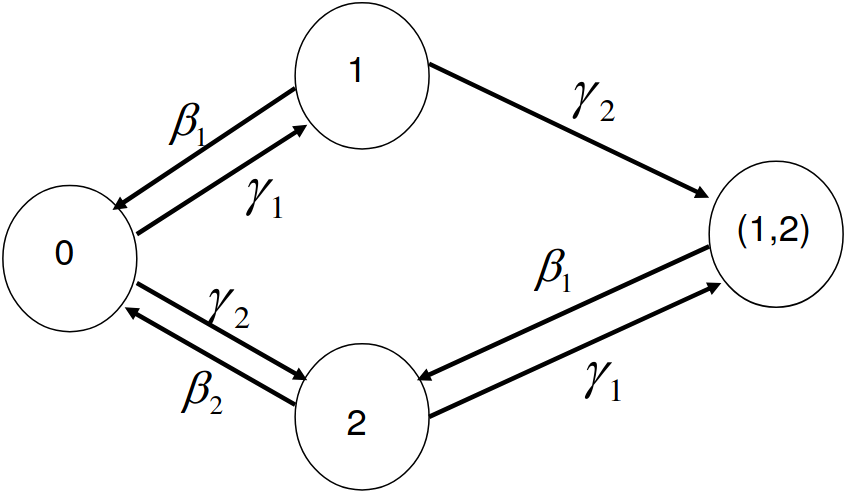
\includegraphics[width=0.35\textwidth]{ctmc_2.png} 
	\end{figure}
	\begin{enumerate}
		\vspace{-.5cm}
		\item[4.] \textit{[6 points]} Suppose that the failure rates are $\gamma_1 = 1$ per month and $\gamma_2 = 3$ per month; and suppose the repair rates are $\beta_1 = 2$ per month and $\beta_2 = 4$ per month.
		Write down some equations(s) to retrieve a/the stationary distribution of this CTMC. Explain why it is solvable.
		\item[5.] \textit{[5 points]} Give an expression of the long-run proportion of time that copier 1 is working.
	\end{enumerate}
	
	
	
	
	
	\newpage
	
	
	%\textcolor{white}{nada}
	
	%\newpage
	
	\maketitle
	
	\begin{center}
		\huge{	DO NOT TURN THIS PAGE OVER UNTIL YOU ARE ALLOWED TO DO SO}
	\end{center}
	
	\thispagestyle{empty} 
	\bigskip
	
	%\paragraph{General guidance :}
	\begin{enumerate}
		\item This is a closed book exam. 
		One A4 page with notes in your own handwriting is allowed.
		\item \textbf{DO NOT} write you name elsewhere other than at the bottom of this page.
		\item Cheating is a \textbf{non-negotiable breach} that will lead to severe penalties.	
		%\item You may assume all of the results presented in class unless explicitly asked for proof.
		%\item Write your solutions in the space provided. If you need more space, write on the last page. %of the problem. Please keep your entire answer to a problem on that problem's pages.
		\item \textbf{Show your work}. Even if your final answer is wrong or you can't finalize it, valid reasoning can get partial credit. 
		Besides, correct answers with erroneous reasoning won't get full credit.
		\item \textbf{Write legibly}. If it can't be read, it can't be graded.
		\item If you get stuck on a question, move on to others. 
		\textbf{Questions are not in order of difficulty}.
		You'll figure out what order they're in once you're done.
		%\item When asked to give a probability distribution, \textbf{make sure to specify the range over which the formula holds}.
		\item When asked to prove a given result, \textbf{be rigorous}. Approximate or \textbf{dishonest attempts to reach a result will be penalized}.
		%\item Please resist the urge to roll on the floor laughing out loud.
		
		\item Questions are repeated in pages $3$ to $13$. Write your solutions in the space provided.
		\item You have \underline{\textbf{two hours and 10 minutes}} to complete the exam.
	\end{enumerate}
	
	\bigskip
	\begin{center}
		\renewcommand{\arraystretch}{2.5} 
		\begin{tabular}{|c|c|c|c|}
			\hline
			\textbf{Attribute} & \textbf{Exercise} & \textbf{Problem}  & \textbf{\quad Total\quad}  \\
			\hline
			\textbf{Questions} & 3 & 13 & 16  \\
			\hline
			\textbf{Points} & 15 & 60 &  75 \\
			\hline
			\textbf{Score} & &  & \\
			\hline
		\end{tabular}
		
	\end{center}
	
	\bigskip
	
	\bigskip
	
	\bigskip
	
	\begin{center}
		\Large{\textbf{Full name : }} $\ldots\ldots\ldots\ldots\ldots\ldots\ldots\ldots\ldots\ldots\ldots\ldots\ldots\ldots$
	\end{center}
	
	\iffalse
	\stepcounter{num} 
	%https://math.mit.edu/classes/18.445/18445all/pset-solutions/Pset3_solutions.pdf
	%page 4
	\paragraph{Part \thenum.}
	A simplified model for the spread of a rumor goes this way: there are $N = 5$ people in a group of friends, of which some have heard the rumor
	and others have not. 
	During any single period of time two people are selected at random
	from the group and assumed to interact. 
	The selection is such that an encounter between any pair of friends is just as likely as any other pair. 
	If one of these persons has heard the rumor and the other has not, then with probability $\alpha = 0.1$ the rumor is transmitted. 
	Let $X_n$ be the number of friends who have heard the rumor at time $n$. 
	
	\begin{enumerate}
		\item Assuming that the process begins at time 0 with a single person knowing the rumor, what is the mean time that it takes for everyone to hear it?
		
		
		
		The rumor has now spread too much and the pilot wants to request an emergency landing for excessive agitation in cabin.
		Consider the problem of sending a binary message, 0 or 1, through a signal
		channel consisting of several stages, where transmission through each stage is
		subject to a fixed probability of error $\alpha$. Suppose that $X_0 = 0$ is the signal that is
		sent and let $X_n$ be the signal that is received at the $n$-th stage. Assume that $\{X_n\}$ is a Markov chain.
		\item Give its transition matrix.
		%transition probabilities $q_{00} = q_{11} = 1 - \alpha$ and $q_{01} =
		%P_{10} = \alpha$, where $0 < \alpha < 1$.
		
		\item Determine $\Pr\{X_0 = 0, X_1 = 0, X_2 = 0\}$, the probability that no error occurs up to stage $n = 2$.
		
		\item Determine the probability that a correct signal is received after 5 transmission stages.
		
		\item 
	\end{enumerate}
	\fi
	
	
\end{document}